\documentclass{article}
\usepackage{tikz}
\usetikzlibrary{positioning}
\usetikzlibrary{shapes.geometric}
\usetikzlibrary{shapes.symbols}
\usetikzlibrary{shadows}
\usetikzlibrary{arrows}

\pagestyle{empty}

\newcommand{\bnstyle}[0]{
  \tikzstyle{var}=[circle,draw] 
  \tikzstyle{dep}=[draw,thick,bend angle=45] }

\newcommand{\nodes}[0]{
  \node [var] (x1) {$x_1$};
  \node [var] (x3) [below=of x1] {$x_3$};
  \node [var] (x2) [left=of x3] {$x_2$};
  \node [var] (x4) [right=of x3] {$x_4$};
  \node [var] (x5) [below=of x3] {$x_5$}; }

\newcommand{\somearcs}[0]{
  \draw [dep, ->, bend right]  (x1) to (x2);
  \draw [dep, ->]                (x1) to (x3);
  \draw [dep, ->, bend left] (x1) to (x4); }

\newcommand{\subnet}[2]{
  \begin{scope}[shift={#1}]
  \nodes
  \somearcs
  #2
  \end{scope} }


\begin{document}

\def\shift{6}

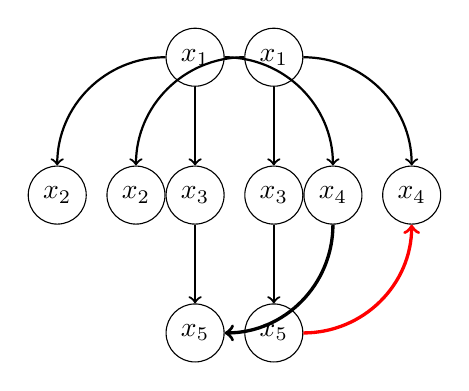
\begin{tikzpicture}
\bnstyle

\subnet{(0,0)}{
   \draw [dep, ->] (x3) to (x5); 
   \draw [dep, ->, bend left=45,very thick] (x4) to (x5); }

\subnet{(\shift,0)}{
   \draw [dep, ->] (x3) to (x5);
   \draw [dep, ->, bend right=45,draw=red,very thick] (x5) to (x4); }
\end{tikzpicture}
\end{document}
